\documentclass{article}
\usepackage{subcaption}
\usepackage[labelformat=parens,labelsep=quad, skip=3pt]{caption}
\usepackage{graphicx}
\usepackage[font=small,labelfont=bf]{caption}
\usepackage{geometry}

\geometry{
 a4paper,
 left=0mm,
 top=0mm,
 }

\begin{document}


\begin{figure}[htp]
 \centering
\begin{subfigure}{.33\textwidth}
 \caption{$\Delta$pCO$_2$ - cGEnIE}
 \includegraphics[width=0.95\linewidth]{../separate_figures/BIOGEM/atm_dpCO2.png}
 \label{fig:dpCO2_1}
\end{subfigure}%
\begin{subfigure}{.33\textwidth}
 \caption{$\Delta$pCO$_2$ - EcoGEnIE}
 \includegraphics[width=0.95\linewidth]{../separate_figures/ECOGEM/atm_dpCO2.png}
 \label{fig:dpCO2_2}
\end{subfigure}
\\[+0.2cm]
\begin{subfigure}{.5\textwidth}
 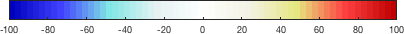
\includegraphics[width=0.95\linewidth]{../separate_figures/ECOGEM/atm_dpCO2_clrbr.png}
\end{subfigure}
\end{figure}


\end{document}